\subsection*{6.1.6 Komponentengraph}
\begin{center}
\begin{tikzpicture}[->, semithick,auto, node distance=2cm]


\node[draw, circle, fill=\sfill] (s) at (0,0) {s};
\node[draw, circle, fill=\Afill] (A) [right of=s] {A};
\node[draw, circle, fill=\Bfill] (B) [below of=A] {B};
\node[draw, circle, fill=\Cfill] (C) [below of=B] {C};
\node[draw, circle, fill=\Dfill] (D) [right of=A] {D};
\node[draw, circle, fill=\Efill] (E) [below of=D] {E};
\node[draw, circle, fill=\Ffill] (F) [below of=E] {F};
\node[draw, circle, fill=\Gfill] (G) [right of=E] {G};

\path 	(s) 	edge node {1} (A)
		edge node {4} (B)
		edge node {9} (C)
	(A) 	edge node {1} (D)
		edge node {5} (E)
	(B) 	edge node {5} (A)
		edge node {2} (E)
	(C) 	edge node {1} (B)
		edge node {6} (F)
	(D) 	edge node {1} (B)
		edge node {15} (G)
	(E) 	edge node {3} (C)
	(F) 	edge node {1} (G)
	(G) 	edge node {4} (E)
	;

\end{tikzpicture}


\end{center}
Der Komponentengraph aus dem obigen Graphen sind wie folgt aus:
\begin{center}
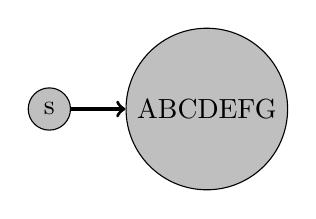
\begin{tikzpicture}[->,node distance=2cm]
\node[draw, circle, fill=lightgray] (s) at (0,0) {s};
\node[draw, circle, fill=lightgray] (abcdefg) [right of=s] {ABCDEFG};

\draw[->, very thick] (s) -- (abcdefg);
\end{tikzpicture}
\end{center}